\documentclass{article}
\usepackage{enumerate}
\usepackage{amsmath}
\usepackage{amssymb}
\usepackage{graphicx}
\usepackage{subfigure}
\usepackage{geometry}
\usepackage{caption}
\usepackage{indentfirst}

\usepackage{algorithm}  
\usepackage{algorithmicx}  
\usepackage{algpseudocode}
\renewcommand{\algorithmicrequire}{\textbf{Input:}}  
\renewcommand{\algorithmicensure}{\textbf{Output:}}  
\usepackage{minted}
\usemintedstyle{autumn}
\setminted{linenos,breaklines,tabsize=4,xleftmargin=1.5em}

\geometry{left=3.0cm,right=3.0cm,top=3.0cm,bottom=4.0cm}

\title{VE281 Project Two Report}
\author{Liu Yihao 515370910207}
\date{}

\begin{document}
\maketitle

\section{Introduction}

In order to study the performances of these two sorting algorithms, I generated different size of arrays and compared the running speed of them (including the std::nth\_element function in STL). Since it's a waste of time to wrote a comparison script written in C++, I chose node-gyp to build the sorting algorithm into a C++ addon of node, and then wrote some Javascript code to benchmark them. Small size of arrays were run for several times so that the result can be more accurate.

\section{Comparison of algorithms}

The limitation of runtime was set to 1s for all algorithms, so some meaningless and slow running were dropped. Then I used MATLAB to plot two graphs, one of small test cases, and another of all cases.

\subsection{General analysis}

\begin{figure}[!htbp]
\centering
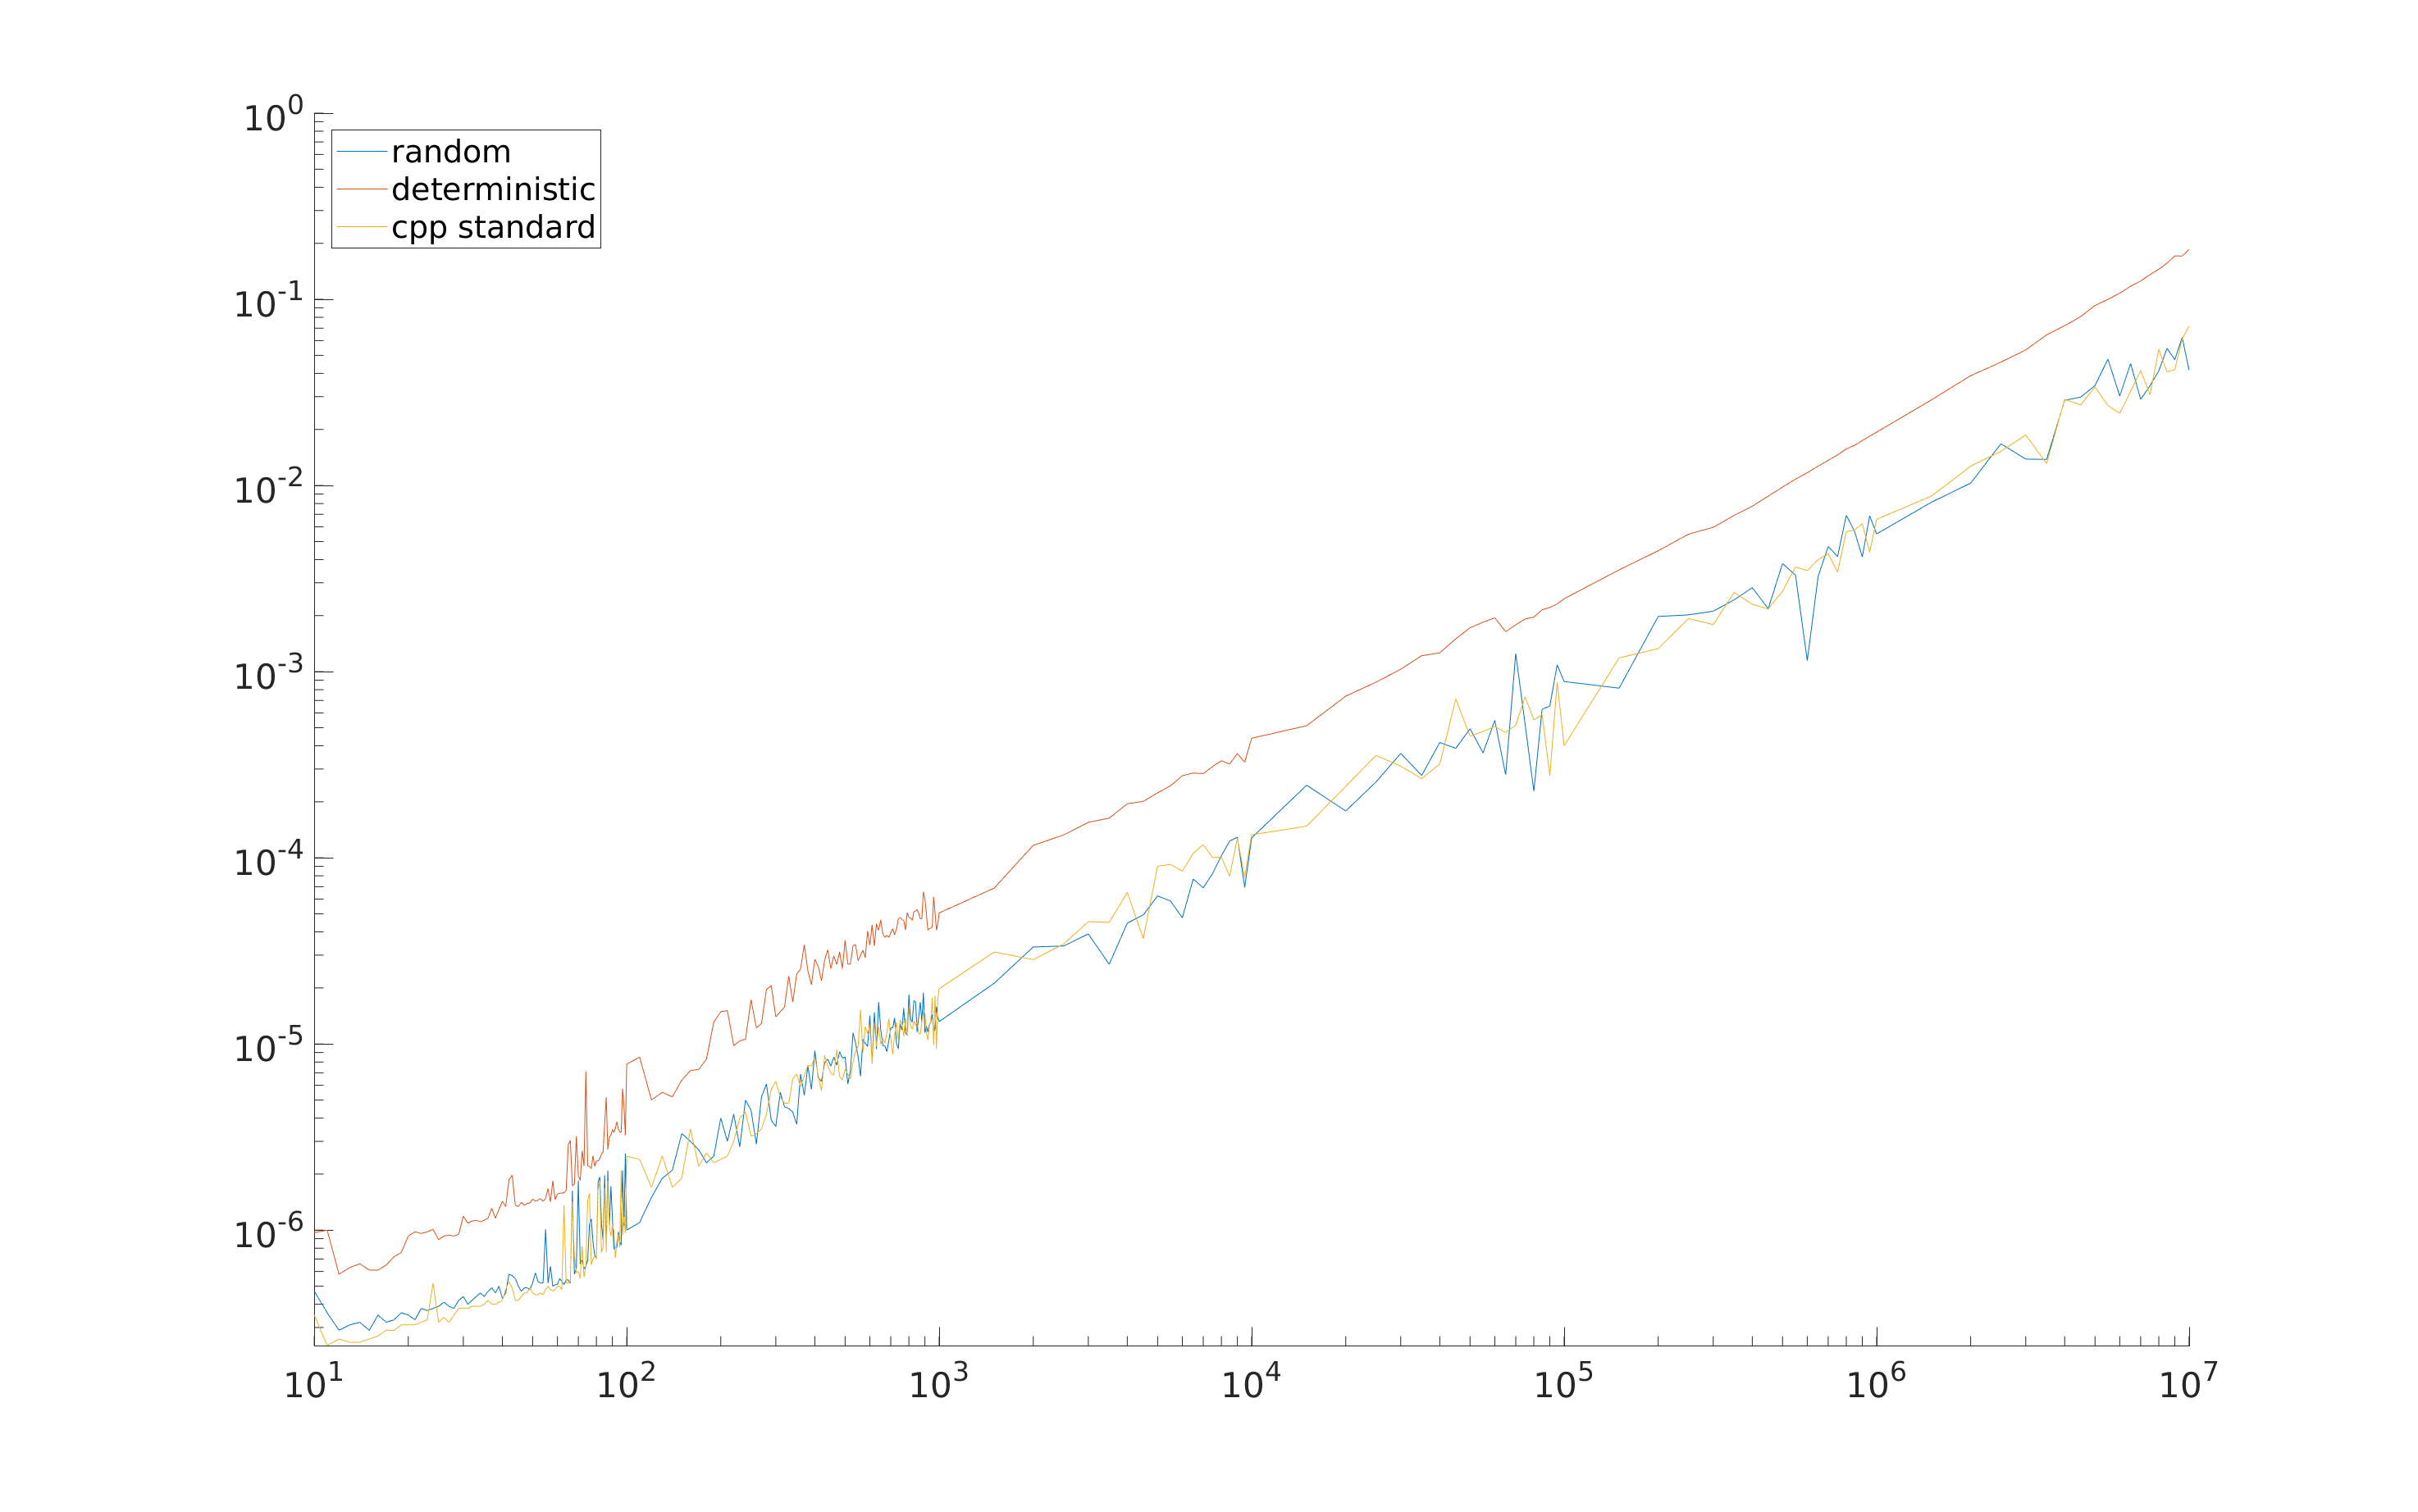
\includegraphics[width=0.8\linewidth]{../benchmark/fig1.png}
\caption{All cases}
\label{fig-1}
\end{figure}

From Figure \ref{fig-1}, we can find that all selections algorithms have the similar running speed. The result satisfy the theory that they have the time complexity of $O(n)$. What's more, deterministic selection is slower than others, which also satisfy with the slides.

\subsection{Small data analysis}

\begin{figure}[!htbp]
\centering
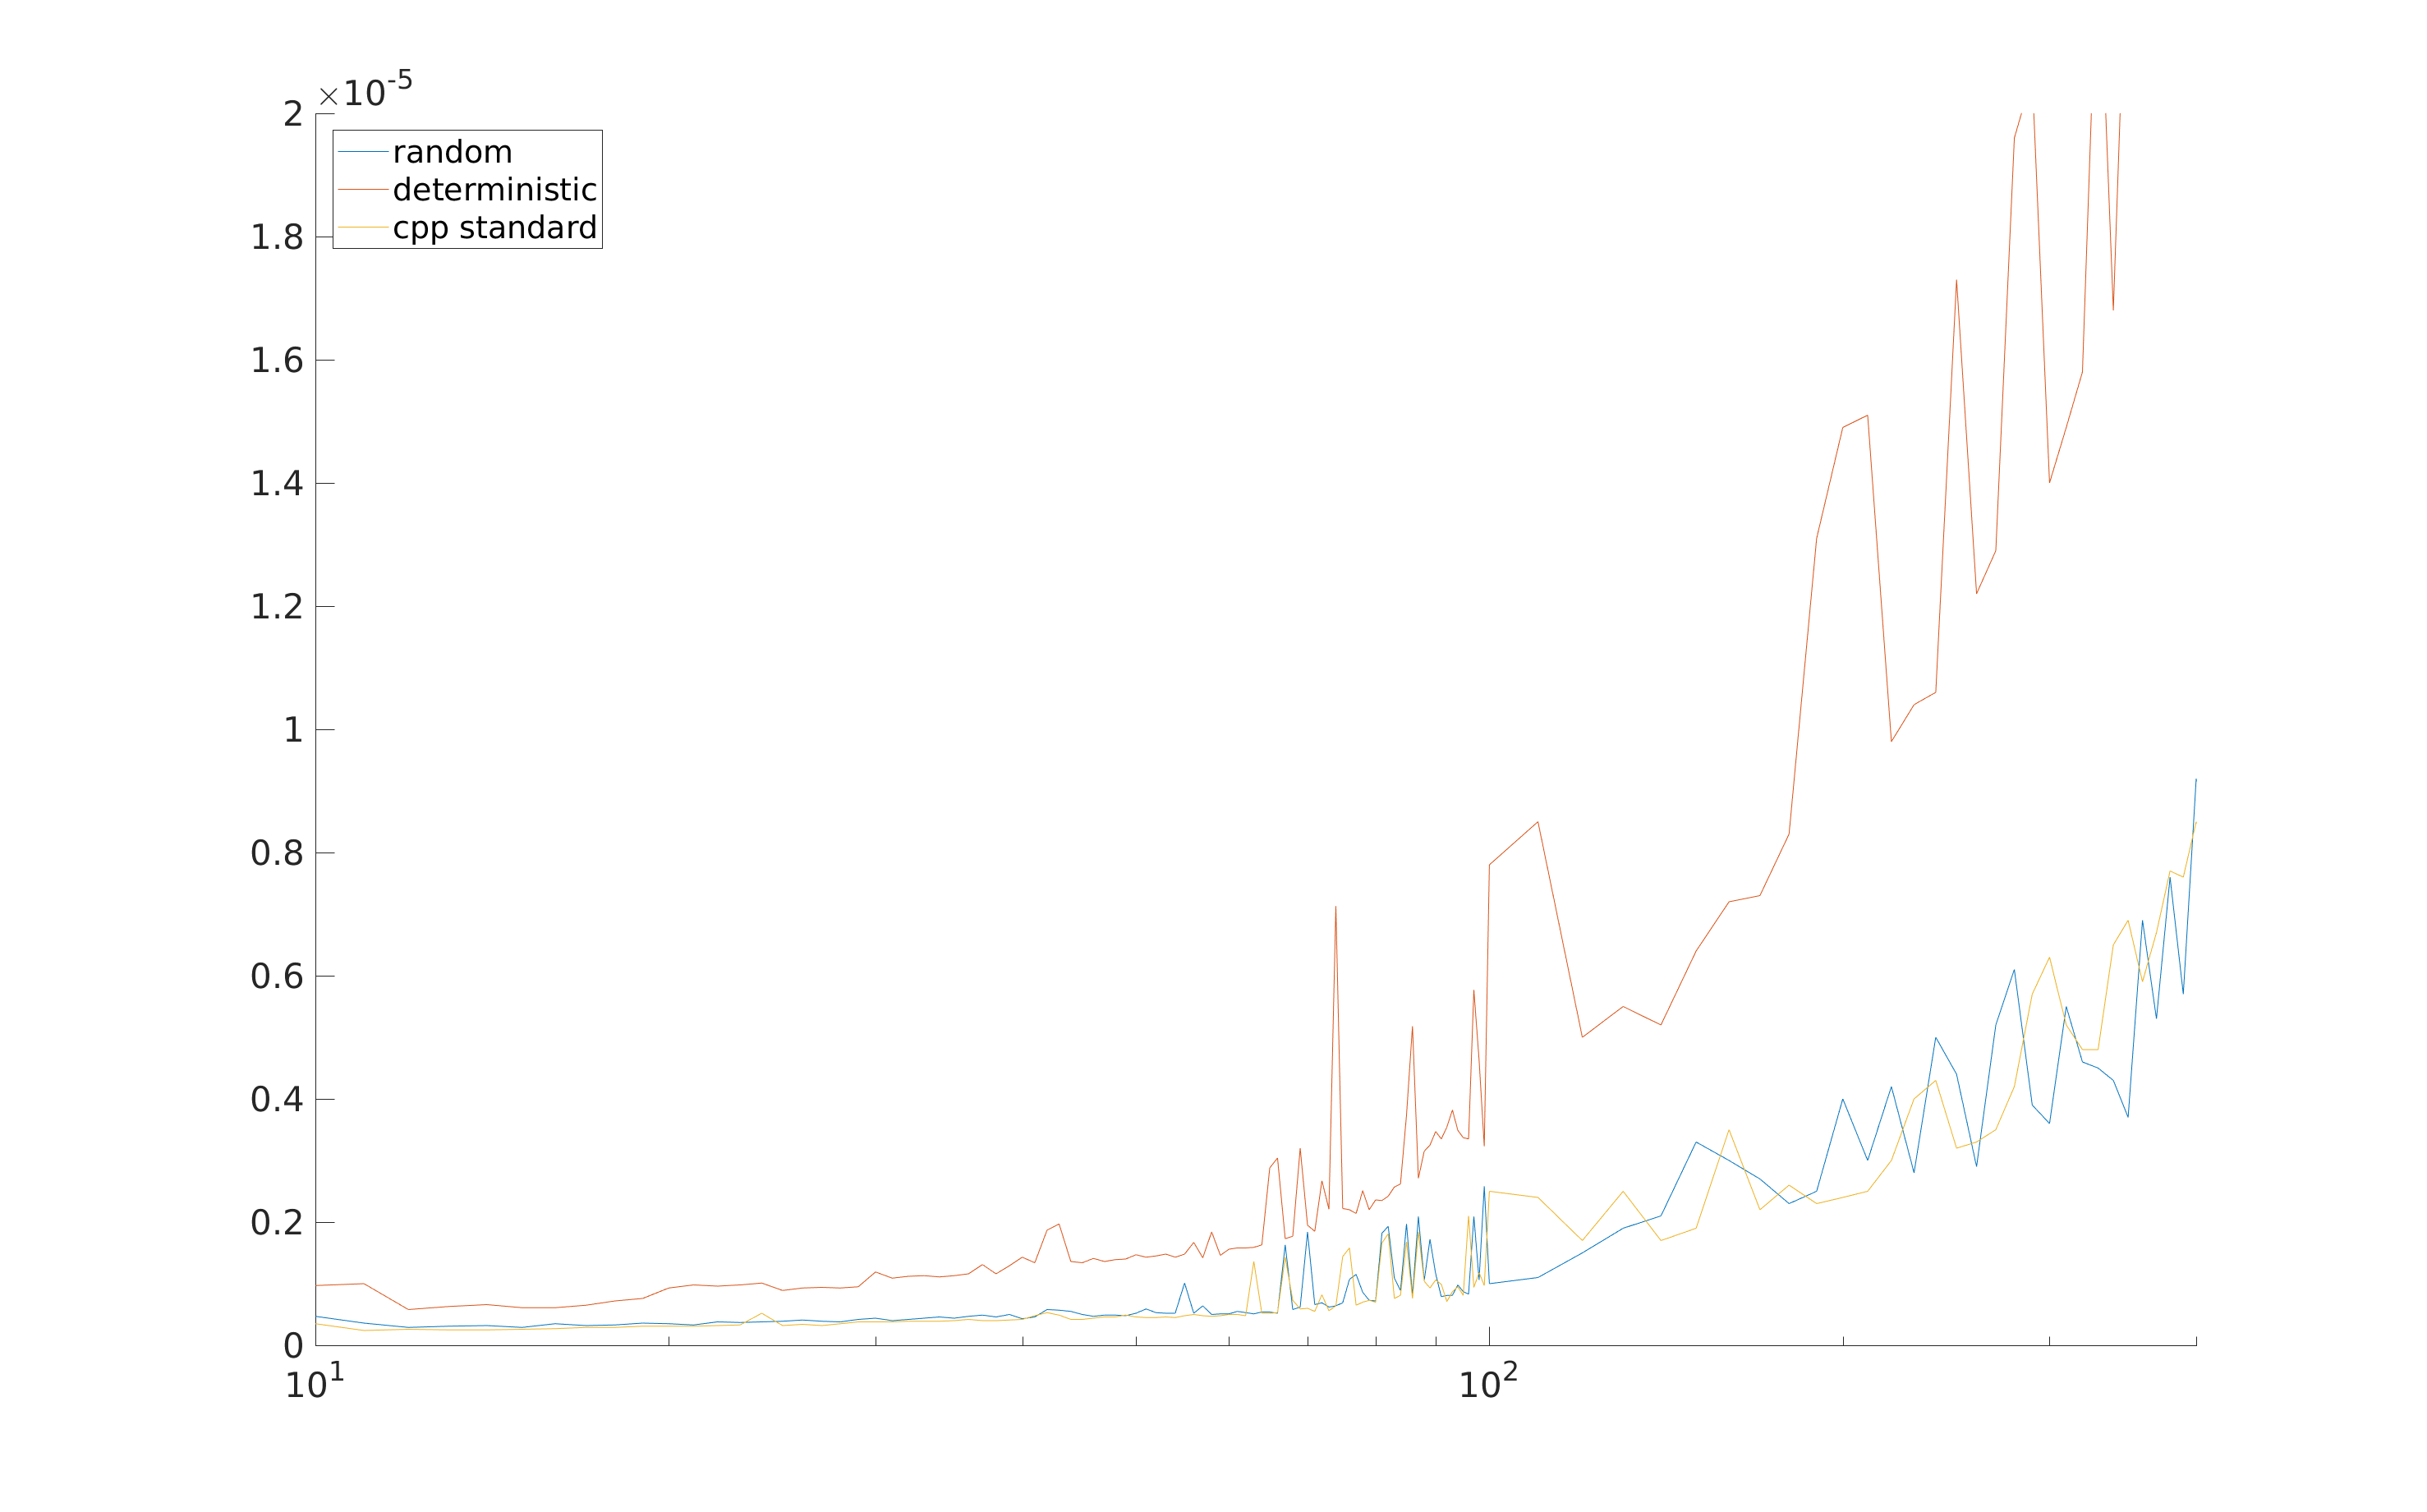
\includegraphics[width=0.8\linewidth]{../benchmark/fig2.png}
\caption{Small cases}
\label{fig-2}
\end{figure}

From Figure \ref{fig-2}, we can find that when the data size is small (from 10 to 100), the comparison of three algorithms are similar to large cases. Now  I can make a guess that the C++ standard selection algorithm is the same as random selection.

\newpage

\section{Appendix}

\subsection{The project files}

\subsubsection{sort.h}
\inputminted{c++}{../answer/selection.h}
\subsubsection{sort.cpp}
\inputminted{c++}{../answer/selection.cpp}
\subsubsection{main.cpp}
\inputminted{c++}{../answer/main.cpp}
\subsubsection{Makefile}
\inputminted{makefile}{../answer/Makefile}


\subsection{The benchmark program}
\subsubsection{README.md}
\inputminted{md}{../benchmark/README.md}
\subsubsection{sort\_wrapper.h}
\inputminted{c++}{../benchmark/selection_wrapper.h}
\subsubsection{sort\_wrapper.cpp}
\inputminted{c++}{../benchmark/selection_wrapper.cpp}
\subsubsection{binding.gyp}
\inputminted{json}{../benchmark/binding.gyp}
\subsubsection{benchmark.js}
\inputminted{javascript}{../benchmark/benchmark.js}
\subsubsection{benchmark.m}
\inputminted{matlab}{../benchmark/benchmark.m}

\end{document}
